\documentclass[prl,amsmath,amssymb,superscriptaddress,12pt]{revtex4-2}

% You may use additional packages as you see fit
\usepackage{graphicx}
\usepackage{verbatim}
\usepackage{braket}
\usepackage{epsfig}
\usepackage{epstopdf}
\usepackage{amsfonts}
\usepackage{amsthm}
\usepackage{float}
\usepackage{amsmath}
\usepackage{amssymb}
\usepackage{color}
\usepackage[usenames,dvipsnames,svgnames,table]{xcolor}
\usepackage{dsfont} 
\usepackage{color}
\usepackage{grffile}
\usepackage{bm}

% ones I added
\usepackage{hyperref} 
\usepackage{multirow}
\hypersetup{colorlinks=true,linkcolor=NavyBlue,citecolor=BrickRed,urlcolor=NavyBlue}

%end of packages

\begin{document} 

\title{Water Potential Lab Report}
\author{Luyu W.V.K.}
\date{\today}

% What is the solute potential of store bought russet potatoes

\maketitle

\section{Introduction}

Water potential difference is one of the key drivers of liquid movement along with kinematic pressure and surface tension forces.

Given a difference in the concentration of a solution inside and outside a barrier, there will be a driving force to equalize these concentrations.

This driving force is exhibited by movement of water in and out of the cell membrane in attempt to minimize the potential. This behavior is otherwise known as 'osmosis'.

This means that when the solution concentration within the cell is less than that outside, water will be pulled through the cell membrane. Conversely, when the solution concentration outside the cell is greater than inside, water will be excreted from the cell.

Because of this, we expect that when the solution inside and outside the cell are isotonic (of the same concentration), we will observe a negligible mass change. 

\section{Methods and Materials}

In this experiment we used transverse sections of Russett potatoes as our cell samples and sucrose ($C_{12}H_{22}O_{11}$) as our solute. 

The solution was pre-diluted into 1.0M, 0.8M, 0.6M, 0.4M, 0.2M, and 0.0M solutions.

Potatoes were cut into 3cm, 2cm, and 1cm cylindrical slices. After massing them (precise to $\pm 0.01g$), we placed the potato slices into the sucrose solutions before leaving them to soak.

The soaking time was roughly 20 hours (varying by around $\pm 3$ hours between groups). This is adequate time for the full piece to equilibrize, according to literature results  (A. Lenart and J. M Flink, 1984) \cite{https://doi.org/10.1111/j.1365-2621.1984.tb00327.x}.

After soaking, potatoes were removed from the solution, lightly damped using paper towels to remove excess solution (qualitatively controlled). After being damped, they were immediately massed (once again accurate to $\pm 0.01g$).

The experiment was completed as a class (in groups of 2-3). Data collected by each group was combined.

In total, as a class, we collected 3 data replicates for each size, 3 sizes (listed above) per solution concentration, and 5 solution concentrations. This means that each datapoint on the concentration axis is $N=9$ (as sizes were not differentiated in data analysis).
 
\section{Results}

The data collected can be seen in the graph below. The datapoint for the $1M$ solution was excluded since we are interested in the linear portion of the osmosis concentration curve. The relationship between concentration and mass change is known to flatten out at high concentrations\footnote{This may be because of solution entering the cavity formed between the cell wall and cell membrane.} .

\begin{figure}[htb]
    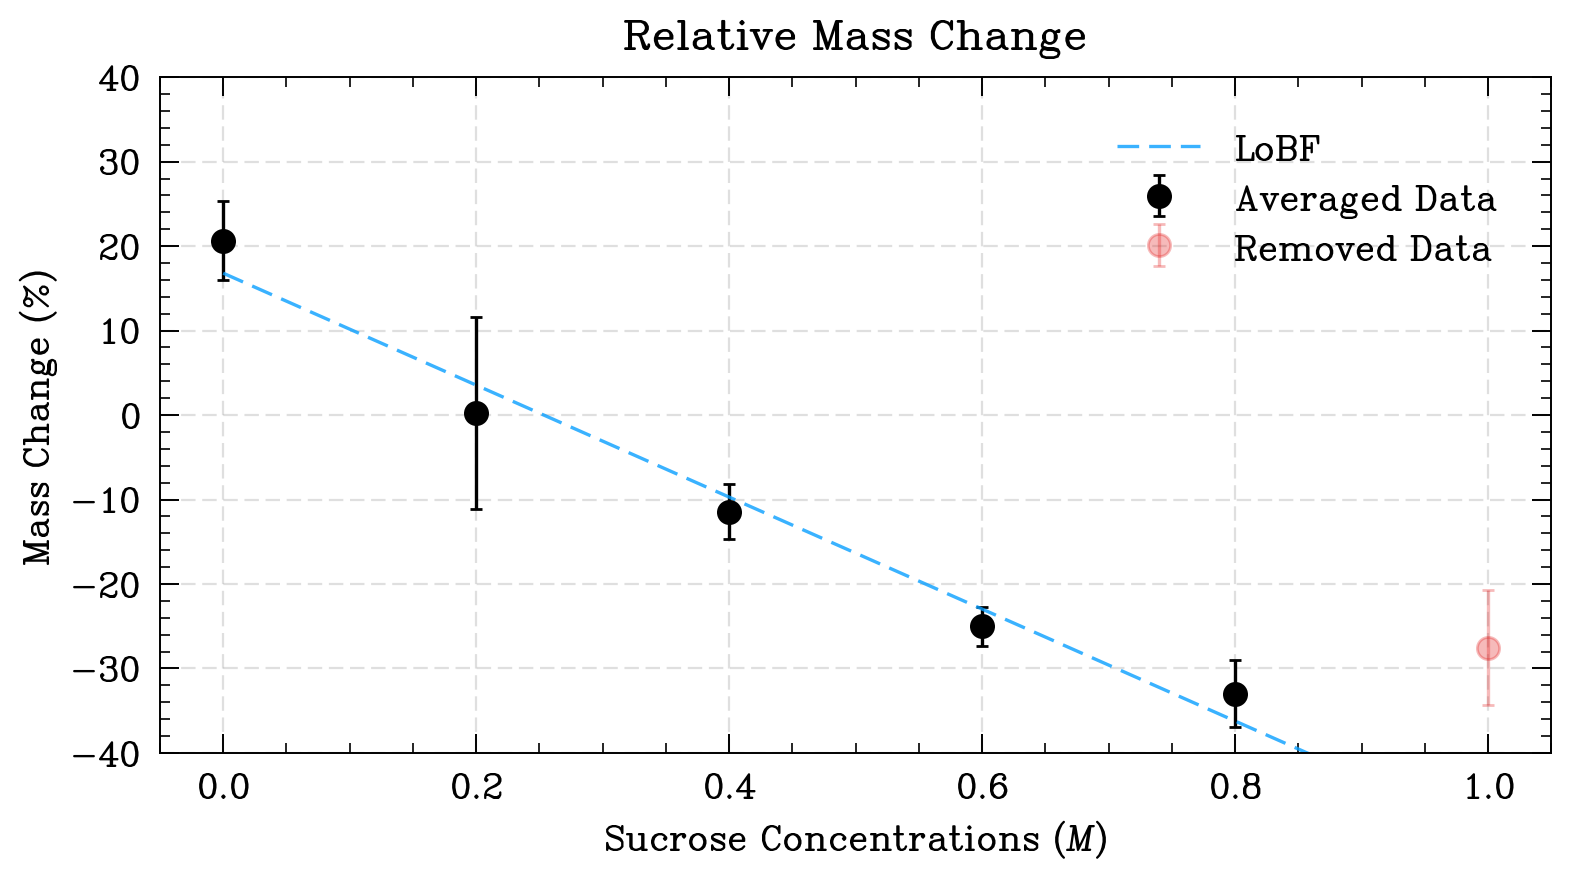
\includegraphics[width=1\linewidth]{lobf.png}
    \caption{Percent mass change in potato in relation to concentration.}
    \label{fig:RelativeMassChange}
\end{figure}

\newpage

To find the osmotic concentration of the potato, we use the $m$ and $b$ values determined through linear regression of our data. 

\begin{equation}
  C_{potato} = -\frac{b}{m}
  \label{eq:solve}
\end{equation}

In this case, our linear regression found $m$ and $b$ values of $-66.3gM^{-1}$ and $16.8g$ respectively. Using Eq. \ref{eq:solve}, we find our osmotic concentration to be $0.25M$.

\section{Discussion}

While the error in our datapoints is cause for disatisfaction, our result nonetheless closely mirrors our hypothesis. There is a clear negative correlation between increasing solution concentration, and the relative mass change. 

Additionally, the mass change crosses from positive (at low sucrose concentrations) to negative (at low sucrose concentrations). This result is consistent to our hypothesis which predicted this to occur at the isotonic concentration. 

Overall, these results clearly point towards water potential as the driving factor in osmosis. 





\bibliography{refs}

\end{document}
